\documentclass{article}

\usepackage[left=2cm,right=2cm, top=2cm, bottom = 2cm]{geometry}
\usepackage{amsfonts}
\usepackage{amsmath}
%%%\usepackage{array}

\usepackage{tikz}

\pagestyle{empty}

\setlength{\tabcolsep}{15pt}
%%%\renewcommand{\arraystretch}{2.5}

%%%\makeatletter
%%%\newcommand{\thickhline}{%
%%%    \noalign {\ifnum 0=`}\fi \hrule height 2pt
%%%    \futurelet \reserved@a \@xhline
%%%}
%%%\newcolumntype{!}{@{\hskip\tabcolsep\vrule width 2pt\hskip\tabcolsep}}
%%%\makeatother

\def\ihat{\hat{\i}}
\def\jhat{\hat{\j}}

\begin{document}

\title{Applications of Compound Angle Formulae}
\date{}

\maketitle
\thispagestyle{empty}

\Large

\textbf{\underline{Objective: To be able to apply compound angle formulae and}}

\textbf{\underline{other trig formulae derived from them to solve problems}}




\vspace{5mm}


\textbf{Recap of previous material:}

\vspace{5mm}

Recall the \textbf{compound angle formulae:}
\[\sin(\alpha+\beta)=\sin(\alpha)\cos(\beta)+\cos(\alpha)\sin(\beta)\]
\[\cos(\alpha+\beta)=\cos(\alpha)\cos(\beta)-\sin(\alpha)\sin(\beta)\]
\[\tan(\alpha+\beta)=\frac{\tan(\alpha)+\tan(\beta)}{1-\tan(\alpha)\tan(\beta)}\]


\begin{enumerate}
\item $\sin\left(\frac{\pi}{3}\right)=$
\item $\cos(\pi)=$
\item $\sin\left(\frac{4\pi}{3}\right)=$
\item $\cos\left(\frac{4\pi}{3}\right)=$
\item $\tan\left(\frac{\pi}{3}\right)=$
\item $\tan\left(\frac{-\pi}{4}\right)=$
\item $\tan\left(\frac{\pi}{12}\right)=$
\item $\sin(\alpha-\beta)=$
\item $\cos(\alpha-\beta)=$
\item $\tan(\alpha-\beta)=$
\end{enumerate}


\clearpage


\textbf{Warm-up:}

\vspace{5mm}

\begin{enumerate}
\item Write down a formula for $\sin(2\theta)$ in terms of $\sin(\theta)$ and $\cos(\theta)$.
\item \begin{enumerate}
	\item Write down a formula for $\cos(2\theta)$ in terms of $\sin(\theta)$ and $\cos(\theta)$.
	\item Apply the formula $\cos^2(\theta)+\sin^2(\theta)=1$ to eliminate $\sin(\theta)$ from this formula.
	\item Apply the Pythagorean formula again in a different way to your formula from part (a) to eliminate $\cos(\theta)$.
	\end{enumerate}
\item Write down a formula for $\tan(2\theta)$ in terms of $\tan(\theta)$.
\item \begin{enumerate}
	\item Express $\sin(3\theta)$ in terms of $\sin(\theta)$, $\sin(2\theta)$, $\cos(\theta)$, and $\cos(2\theta)$.
	\item Hence express $\sin(3\theta)$ in terms of $\sin(\theta)$ and $\cos(\theta)$ only.
	\item Eliminate $\cos(\theta)$ to obtain an expression for $\sin(3\theta)$ in terms of $\sin(\theta)$ only.
	\end{enumerate}
\item Apply the compound angle formula for cosine to the expression
\[\cos(\alpha+\beta) + \cos(\alpha-\beta).\]
\item Apply the compound angle formula for cosine to the expression
\[\cos(\alpha-\beta) - \cos(\alpha+\beta).\]
\end{enumerate}




\clearpage

\textbf{Theory---Products of Sinusoids:}

\vspace{5mm}

We shall explore how to use the compound angle formulae ``backwards'' to deal with products of sinusoids. We saw in the last two questions of the warm-up that:
\[\cos(\alpha)\cos(\beta)=\frac{1}{2}\left(\cos(\alpha+\beta)+\cos(\alpha-\beta)\right)\]
\[\sin(\alpha)\sin(\beta)=\frac{1}{2}\left(\cos(\alpha-\beta)-\cos(\alpha+\beta)\right).\]

These formulae allow us to transform a product of two sines or of two cosines into a sum of cosines:

\vspace{5mm}

Write $\cos(3\pi t)\cos(10\pi t)$ as a sum of sinusoids:

\vfill

Write $6\sin\left(\pi t+\frac{\pi}{3}\right)\sin(5\pi t)$ as a sum of sinusoids:

\vfill

Note: these formulae only directly tell us how to deal with the product of two sines or two cosines. But any sinusoid can be turned into a sine (or a cosine) with a phase shift, so this covers any product of two sinusoid functions.


\clearpage


Here we show graphs of the functions from the last page:

\begin{center}
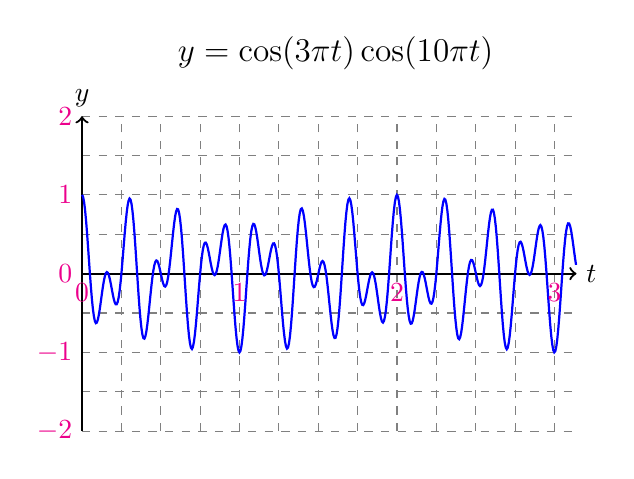
\begin{tikzpicture}
\draw[step=0.5,gray,thin,dashed] (0,-2) grid (6.28,2);
\draw[thick, ->] (0,-2) -- (0,2);
\node[above] at (0,2) {$y$};
\draw[thick,->] (0,0) -- (6.28,0);
\node[right] at (6.28,0) {$t$};

\draw[blue,thick, domain=0:6.28, samples=500] plot (\x,{0.5*cos(20.42*\x r) + 0.5*cos(11*\x r)});

\node[magenta,below] at (0,0) {0};
\node[magenta,below] at (2,0) {1};
\node[magenta,below] at (4,0) {2};
\node[magenta,below] at (6,0) {3};

\node[above,font=\large] at (current bounding box.north) {$y=\cos(3\pi t)\cos(10\pi t)$};

\foreach \i in {-2,-1,0,1,2}{
	\node[left,magenta] at (0,\i) {$\i$};
	}
\end{tikzpicture}
\end{center}

\vfill

\begin{center}
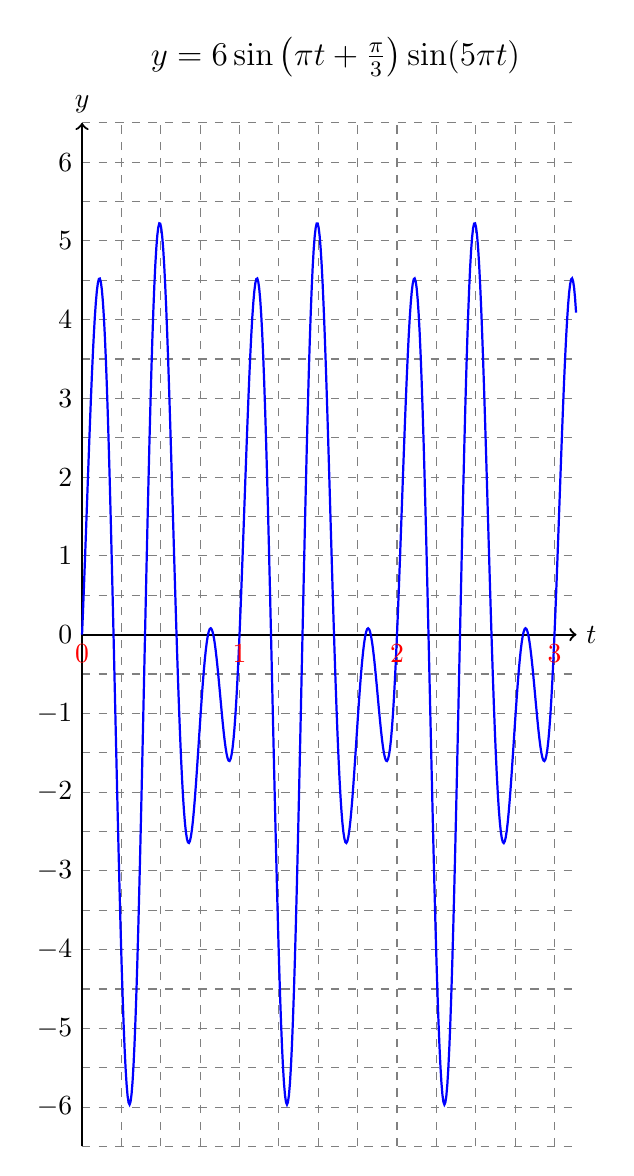
\begin{tikzpicture}
\draw[step=0.5,gray,thin,dashed] (0,-6.5) grid (6.28,6.5);
\draw[thick, ->] (0,-6.5) -- (0,6.5);
\node[above] at (0,6.5) {$y$};
\draw[thick,->] (0,0) -- (6.28,0);
\node[right] at (6.28,0) {$t$};

\draw[blue,thick, domain=0:6.28, samples=500] plot (\x,{3*cos((2*pi*\x - (pi/6)) r) - 3*cos((3*pi*\x+(pi/6)) r)});

\node[red,below] at (0,0) {0};
\node[red,below] at (2,0) {1};
\node[red,below] at (4,0) {2};
\node[red,below] at (6,0) {3};

\node[above,font=\large] at (current bounding box.north) {$y=6\sin\left(\pi t+\frac{\pi}{3}\right)\sin(5\pi t)$};

\foreach \i in {-6,-5,-4,-3,-2,-1,0,1,2,3,4,5,6}{
	\node[left] at (0,\i) {$\i$};
	}
\end{tikzpicture}
\end{center}


\clearpage

\textbf{Theory---Sums of Sinusoids of Equal Frequency:}

\vspace{5mm}

The compound angle formulae split a single sine or cosine into a combination of sines and cosines. We can use this in reverse to combine sines and cosines \textbf{of the same frequency} into a single sine or cosine.

\vspace{5mm}

Write $3\cos(7\theta)-4\sin(7\theta)$ in the form $R\cos(7\theta+\alpha)$ for some $R$ and $\alpha$.

\vfill

Write $\cos\left(2\theta-\frac{\pi}{4}\right)+2\sin(2\theta)$ in the form $R\sin(2\theta +\alpha)$ for some $R$ and $\alpha$.

\vfill



\clearpage



Here we show graphs of the functions from the last page:

\begin{center}
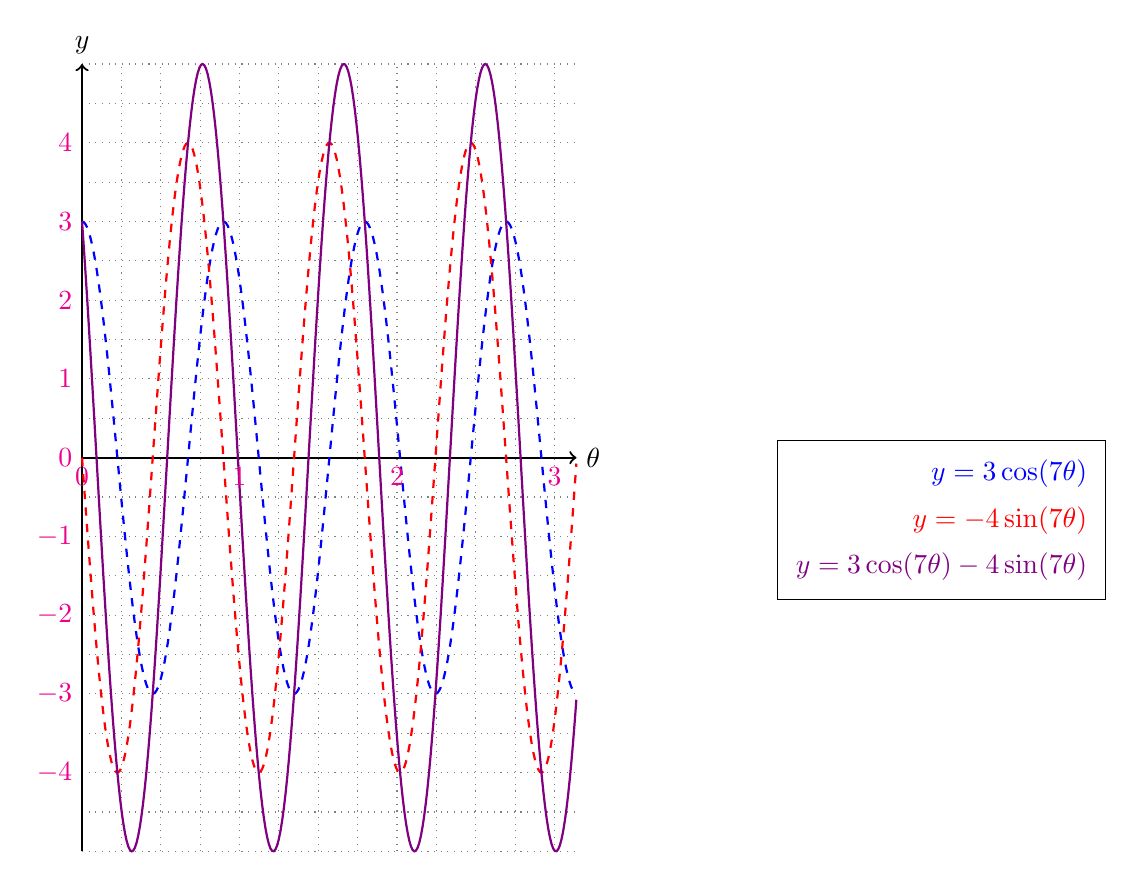
\begin{tikzpicture}
\draw[white] (0,0) -- (13,0);
\draw[step=0.5,gray,thin,dotted] (0,-5) grid (6.28,5);
\draw[thick, ->] (0,-5) -- (0,5);
\node[above] at (0,5) {$y$};
\draw[thick,->] (0,0) -- (6.28,0);
\node[right] at (6.28,0) {$\theta$};

\draw[blue,thick, dashed, domain=0:6.28, samples=300] plot (\x,{3*cos((3.5*\x) r)});
\draw[red,thick, dashed, domain=0:6.28, samples=300] plot (\x,{-4*sin((3.5*\x) r)});
\draw[violet,thick, domain=0:6.28, samples=300] plot (\x,{3*cos((3.5*\x) r) - 4*sin((3.5*\x) r)});

\node[magenta,below] at (0,0) {0};
\node[magenta,below] at (2,0) {1};
\node[magenta,below] at (4,0) {2};
\node[magenta,below] at (6,0) {3};


\foreach \i in {-4,-3,-2,-1,0,1,2,3,4}{
	\node[left,magenta] at (0,\i) {$\i$};
	}
	
\matrix [draw,below left] at (current bounding box.east) {
	\node [blue] {$y=3\cos(7\theta)$}; \\
	\node [red] {$y=-4\sin(7\theta)$}; \\
	\node[violet] {$y=3\cos(7\theta)-4\sin(7\theta)$};\\
};
\end{tikzpicture}
\end{center}

\vfill


\begin{center}
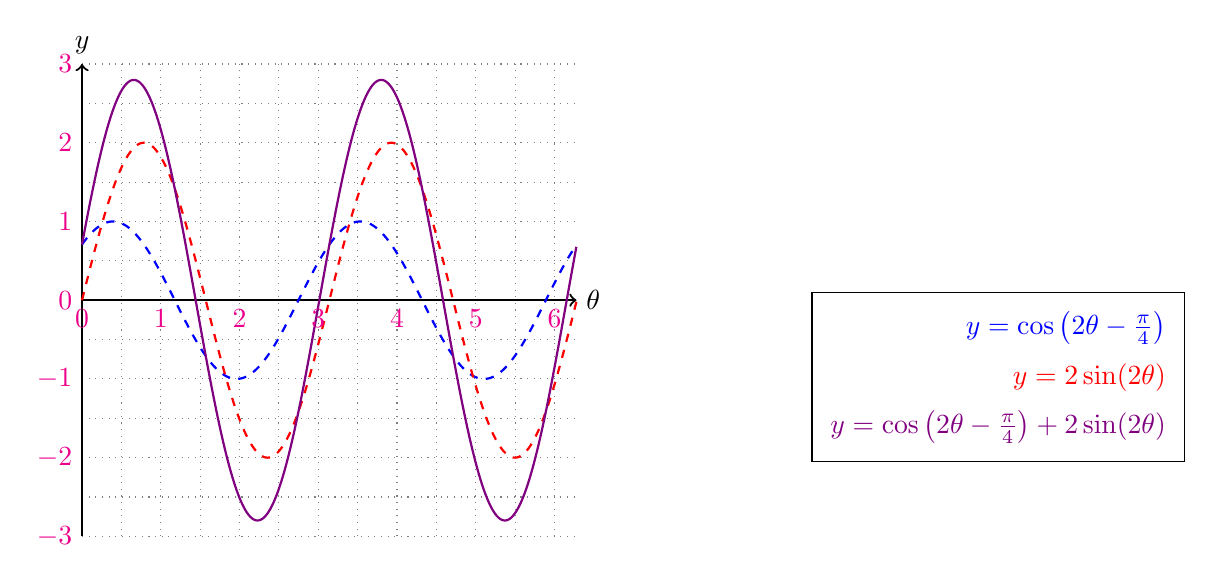
\begin{tikzpicture}
\draw[white] (0,0) -- (14,0);
\draw[step=0.5,gray,thin,dotted] (0,-3) grid (6.28,3);
\draw[thick, ->] (0,-3) -- (0,3);
\node[above] at (0,3) {$y$};
\draw[thick,->] (0,0) -- (6.28,0);
\node[right] at (6.28,0) {$\theta$};

\draw[blue,thick, dashed, domain=0:6.28, samples=300] plot (\x,{cos((2*\x - (pi/4)) r)});
\draw[red,thick, dashed, domain=0:6.28, samples=300] plot (\x,{2*sin((2*\x) r)});
\draw[violet,thick, domain=0:6.28, samples=300] plot (\x,{cos((2*\x - (pi/4)) r) + 2*sin((2*\x) r)});

\foreach \i in {0,1,2,3,4,5,6}{
	\node[below,magenta] at (\i,0) {$\i$};
}


\foreach \i in {-3,-2,-1,0,1,2,3}{
	\node[left,magenta] at (0,\i) {$\i$};
}
	
\matrix [draw,below left] at (current bounding box.east) {
	\node [blue] {$y=\cos\left(2\theta-\frac{\pi}{4}\right)$}; \\
	\node [red] {$y=2\sin(2\theta)$}; \\
	\node[violet] {$y=\cos\left(2\theta-\frac{\pi}{4}\right)+2\sin(2\theta)$};\\
};
\end{tikzpicture}
\end{center}





\clearpage



\textbf{Practice:}

\vspace{5mm}

Recall the \textbf{compound angle formulae:} for sine and cosine:
\[\sin(\alpha+\beta)=\sin(\alpha)\cos(\beta)+\cos(\alpha)\sin(\beta)\]
\[\cos(\alpha+\beta)=\cos(\alpha)\cos(\beta)-\sin(\alpha)\sin(\beta)\]

\begin{enumerate}
\item Write $4\cos(t)\sin(3t)$ as a sum of sinusoids.
\item Write $\sin(5\pi t)\sin(50\pi t)$ as a sum of sinusoids.
\item Write $\sin\left(\pi t+\frac{\pi}{4}\right) + \cos\left(\pi t - \frac{\pi}{6}\right)$ in the form $R\cos(\pi t + \alpha)$.
\end{enumerate}

\clearpage


\textbf{Application---Triple Phase Power:}

\vspace{5mm}

Mains electricity is generated in a 3-phase generator, as this is much more efficient than a single phase generator. This means that three different voltage outputs are produced, each with the same amplitude and frequency, but different phases. These are then transmitted along 4 wires---one for each phase and one at the average (0), called neutral.

Each voltage signal has an amplitude of $230\sqrt{2}\mathrm{V}\approx325\mathrm{V}$ (relative to neutral), a frequency of 50Hz, and a phase shift of $\frac{2\pi}{3}$ relative to the others (so the three phases are $0$, $\frac{2\pi}{3}$, and $\frac{4\pi}{3}$). A lot of more powerful electric motors run from 3-phase supplies; they are wired with their active drive coils connected between phases (A-B, B-C, C-A) in what is called a delta scheme. The factor of $\sqrt{2}$ in the voltage is because mains power has a root mean square voltage of $230\mathrm{V}$.

What is the overall amplitude and phase of voltage across each of the 3 drive coils? What is the root mean square voltage across each drive coil?

\begin{center}
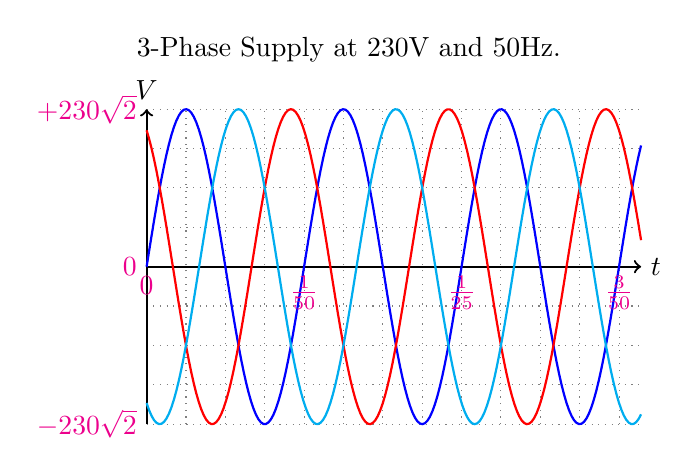
\begin{tikzpicture}
\draw[step=0.5,gray,thin,dotted] (0,-2) grid (6.28,2);
\draw[thick, ->] (0,-2) -- (0,2);
\node[above] at (0,2) {$V$};
\draw[thick,->] (0,0) -- (6.28,0);
\node[right] at (6.28,0) {$t$};

\draw[blue,thick, domain=0:6.28, samples=200] plot (\x,{2*sin((pi*\x) r)});
\draw[red,thick, domain=0:6.28, samples=200] plot (\x,{2*sin((pi*\x + (2*pi/3)) r)});
\draw[cyan,thick, domain=0:6.28, samples=200] plot (\x,{2*sin((pi*\x+(4*pi/3)) r)});


\node[magenta,below] at (0,0) {0};
\node[magenta,below] at (2,0) {$\frac{1}{50}$};
\node[magenta,below] at (4,0) {$\frac{1}{25}$};
\node[magenta,below] at (6,0) {$\frac{3}{50}$};


\node[magenta,left] at (0,0) {$0$};
\node[magenta,left] at (0,-2) {$-230\sqrt{2}$};
\node[magenta,left] at (0,2) {$+230\sqrt{2}$};

\node[above] at (current bounding box.north) {3-Phase Supply at $230$V and $50$Hz.};
\end{tikzpicture}
\end{center}



\clearpage



\textbf{Application---AM Radio:}

\vspace{5mm}

A formerly very common but now fairly obsolete method of transmitting information via radio is amplitude modulation (AM). This is done by using a fixed high frequency `carrier wave.' The sound signal (or other information) is converted to an analogue electrical signal (a sine wave, say), and then the carrier wave is multiplied by the signal.

Assume the carrier wave is $\cos(\omega t)$ and the audio wave is $A\cos(\xi t)$ as functions of time, where $\omega$ and $\xi$ are the relevant frequencies and $A$ is the amplitude of the information signal.

\begin{enumerate}
\item What is the waveform which results from multiplying the carrier wave and information signal together?
\item What can you say about the frequencies and amplitudes that are present in the resulting waveform?
\item What if we phase shift the information signal to $A\cos(\xi t+\phi)$ for some $\phi$? What waveform results then, and what frequencies and amplitudes occur in it?
\end{enumerate}

\begin{center}
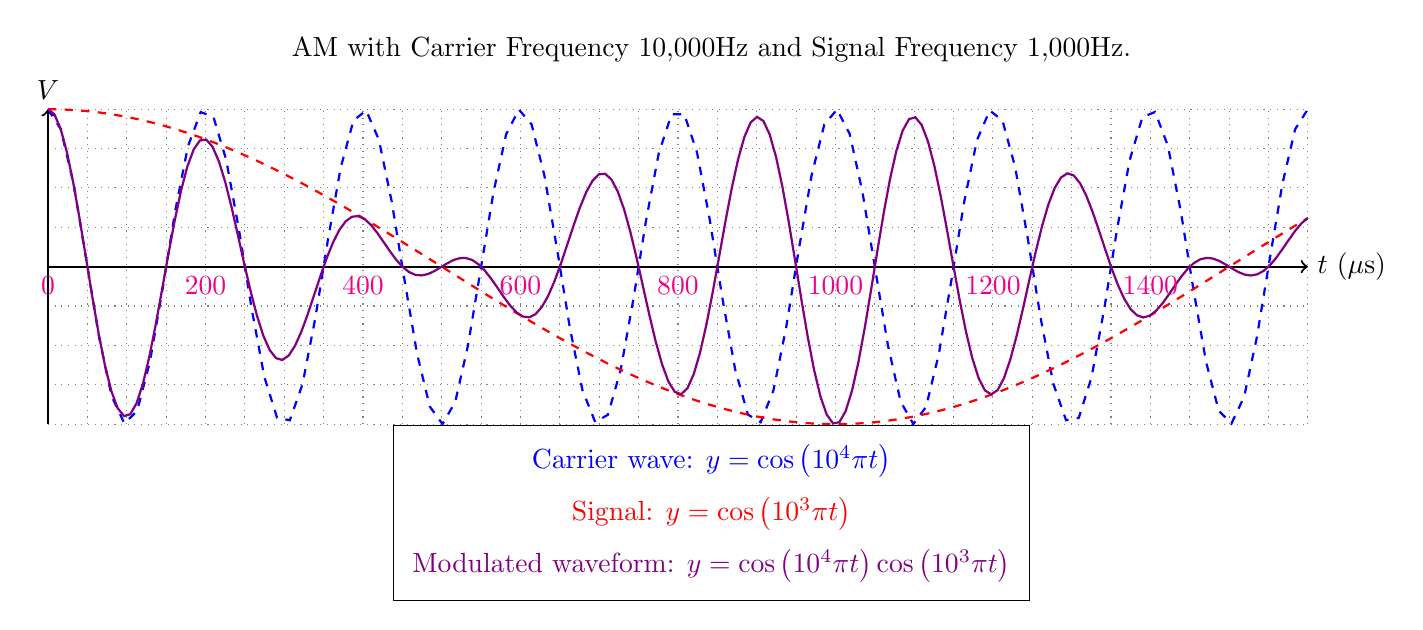
\begin{tikzpicture}
\draw[step=0.5,gray,thin,dotted] (0,-2) grid (16,2);
\draw[thick, ->] (0,-2) -- (0,2);
\node[above] at (0,2) {$V$};
\draw[thick,->] (0,0) -- (16,0);
\node[right] at (16,0) {$t$ ($\mu$s)};

\draw[blue,thick, dashed, domain=0:16, samples=100] plot (\x,{2*cos((pi*\x) r)});
\draw[red,thick, dashed, domain=0:16, samples=100] plot (\x,{2*cos((0.1*pi*\x) r)});
\draw[violet,thick, domain=0:16, samples=200] plot (\x,{2*cos((0.1*pi*\x) r)*cos((pi*\x) r)});

\node[magenta,below] at (0,0) {0};

\foreach \i in {2,4,6,8,10,12,14}{
	\node[magenta,below] at (\i,0) {$\i 00$};
}


\node[above] at (current bounding box.north) {AM with Carrier Frequency 10,000Hz and Signal Frequency 1,000Hz.};

\matrix [draw,below] at (current bounding box.south) {
	\node [blue] {Carrier wave: $y=\cos\left(10^4\pi t\right)$}; \\
	\node [red] {Signal: $y=\cos\left(10^3\pi t\right)$}; \\
	\node[violet] {Modulated waveform: $y=\cos\left(10^4\pi t\right)\cos\left(10^3\pi t\right)$};\\
};
\end{tikzpicture}
\end{center}




\clearpage


\textbf{Key Points to Remember:}

\begin{enumerate}
\item The \textbf{compound angle formulae} for sine and cosine are:
	\[\cos(\alpha+\beta)=\cos(\alpha)\cos(\beta)-\sin(\alpha)\sin(\beta)\]
	\[\sin(\alpha+\beta)=\sin(\alpha)\cos(\beta)+\cos(\alpha)\sin(\beta)\]
\item We can decompose the product of two sines or of two cosines:
	\[\cos(\alpha)\cos(\beta)=\frac{1}{2}\left(\cos(\alpha+\beta)+\cos(\alpha-\beta)\right)\]
	\[\sin(\alpha)\sin(\beta) = \frac{1}{2}\left(\cos(\alpha-\beta)-\cos(\alpha+\beta)\right)\]
\item We can express a sum of sinusoids \textbf{of the same frequency} (and any phase and amplitude) as a single sinusoid:
	\[A\sin(\omega t+\phi)+B\cos(\omega t+\psi) = R\sin(\omega t+\alpha) \mbox{ or } S\cos(\omega t+\beta)\]
	where	$R$ and $\alpha$ (or $S$ and $\beta$) are found by expanding the right-hand side with a compound angle formula and comparing coefficients of $\sin$ and of $\cos$.
\item The sum of sinusoids \textbf{of the same frequency} is a sinusoid. The product of sinusoids, or the sum of sinusoids of different frequencies, is a more complicated waveform.
\end{enumerate}




\end{document}